\chapter{Appendix B. Other Bad Areas}
\label{appb:bad}
\begin{figure*}
  \includegraphics{appendix/B/fig/over_all_overlap.png}               
  \caption[overlay of accidents and `bad reports']{The overlay of accidents in Boston and Cambridge and `bad' reports}
  \label{fig:bad_overlay}
\end{figure*}

\begin{figure}[!htb]
  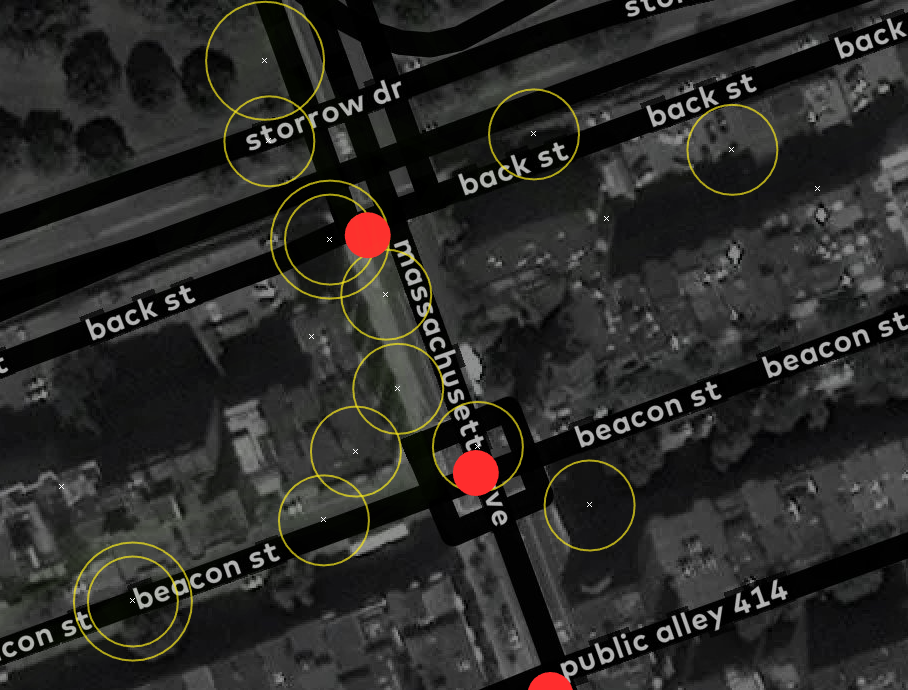
\includegraphics{appendix/B/fig/overlap_beacon.png}               
  \caption[dangerous crossing in Massachusetts Avenue at Beacon Street]{This place was repeadly reported by local news media and considered to be one of the most dangerous areas in Boston. The city responded after a fatal accident in 2015. Beacon street is now a protected bike lane, with the bike lane located right next to the side walk, guarded with parked cars. The result shows that it is still unsafe approaching to this crossing, cars tend to speed up at the bridge rushing to catch the street light.}
  \label{fig:bad_beacon}
\end{figure}

\begin{figure}[!htb]
  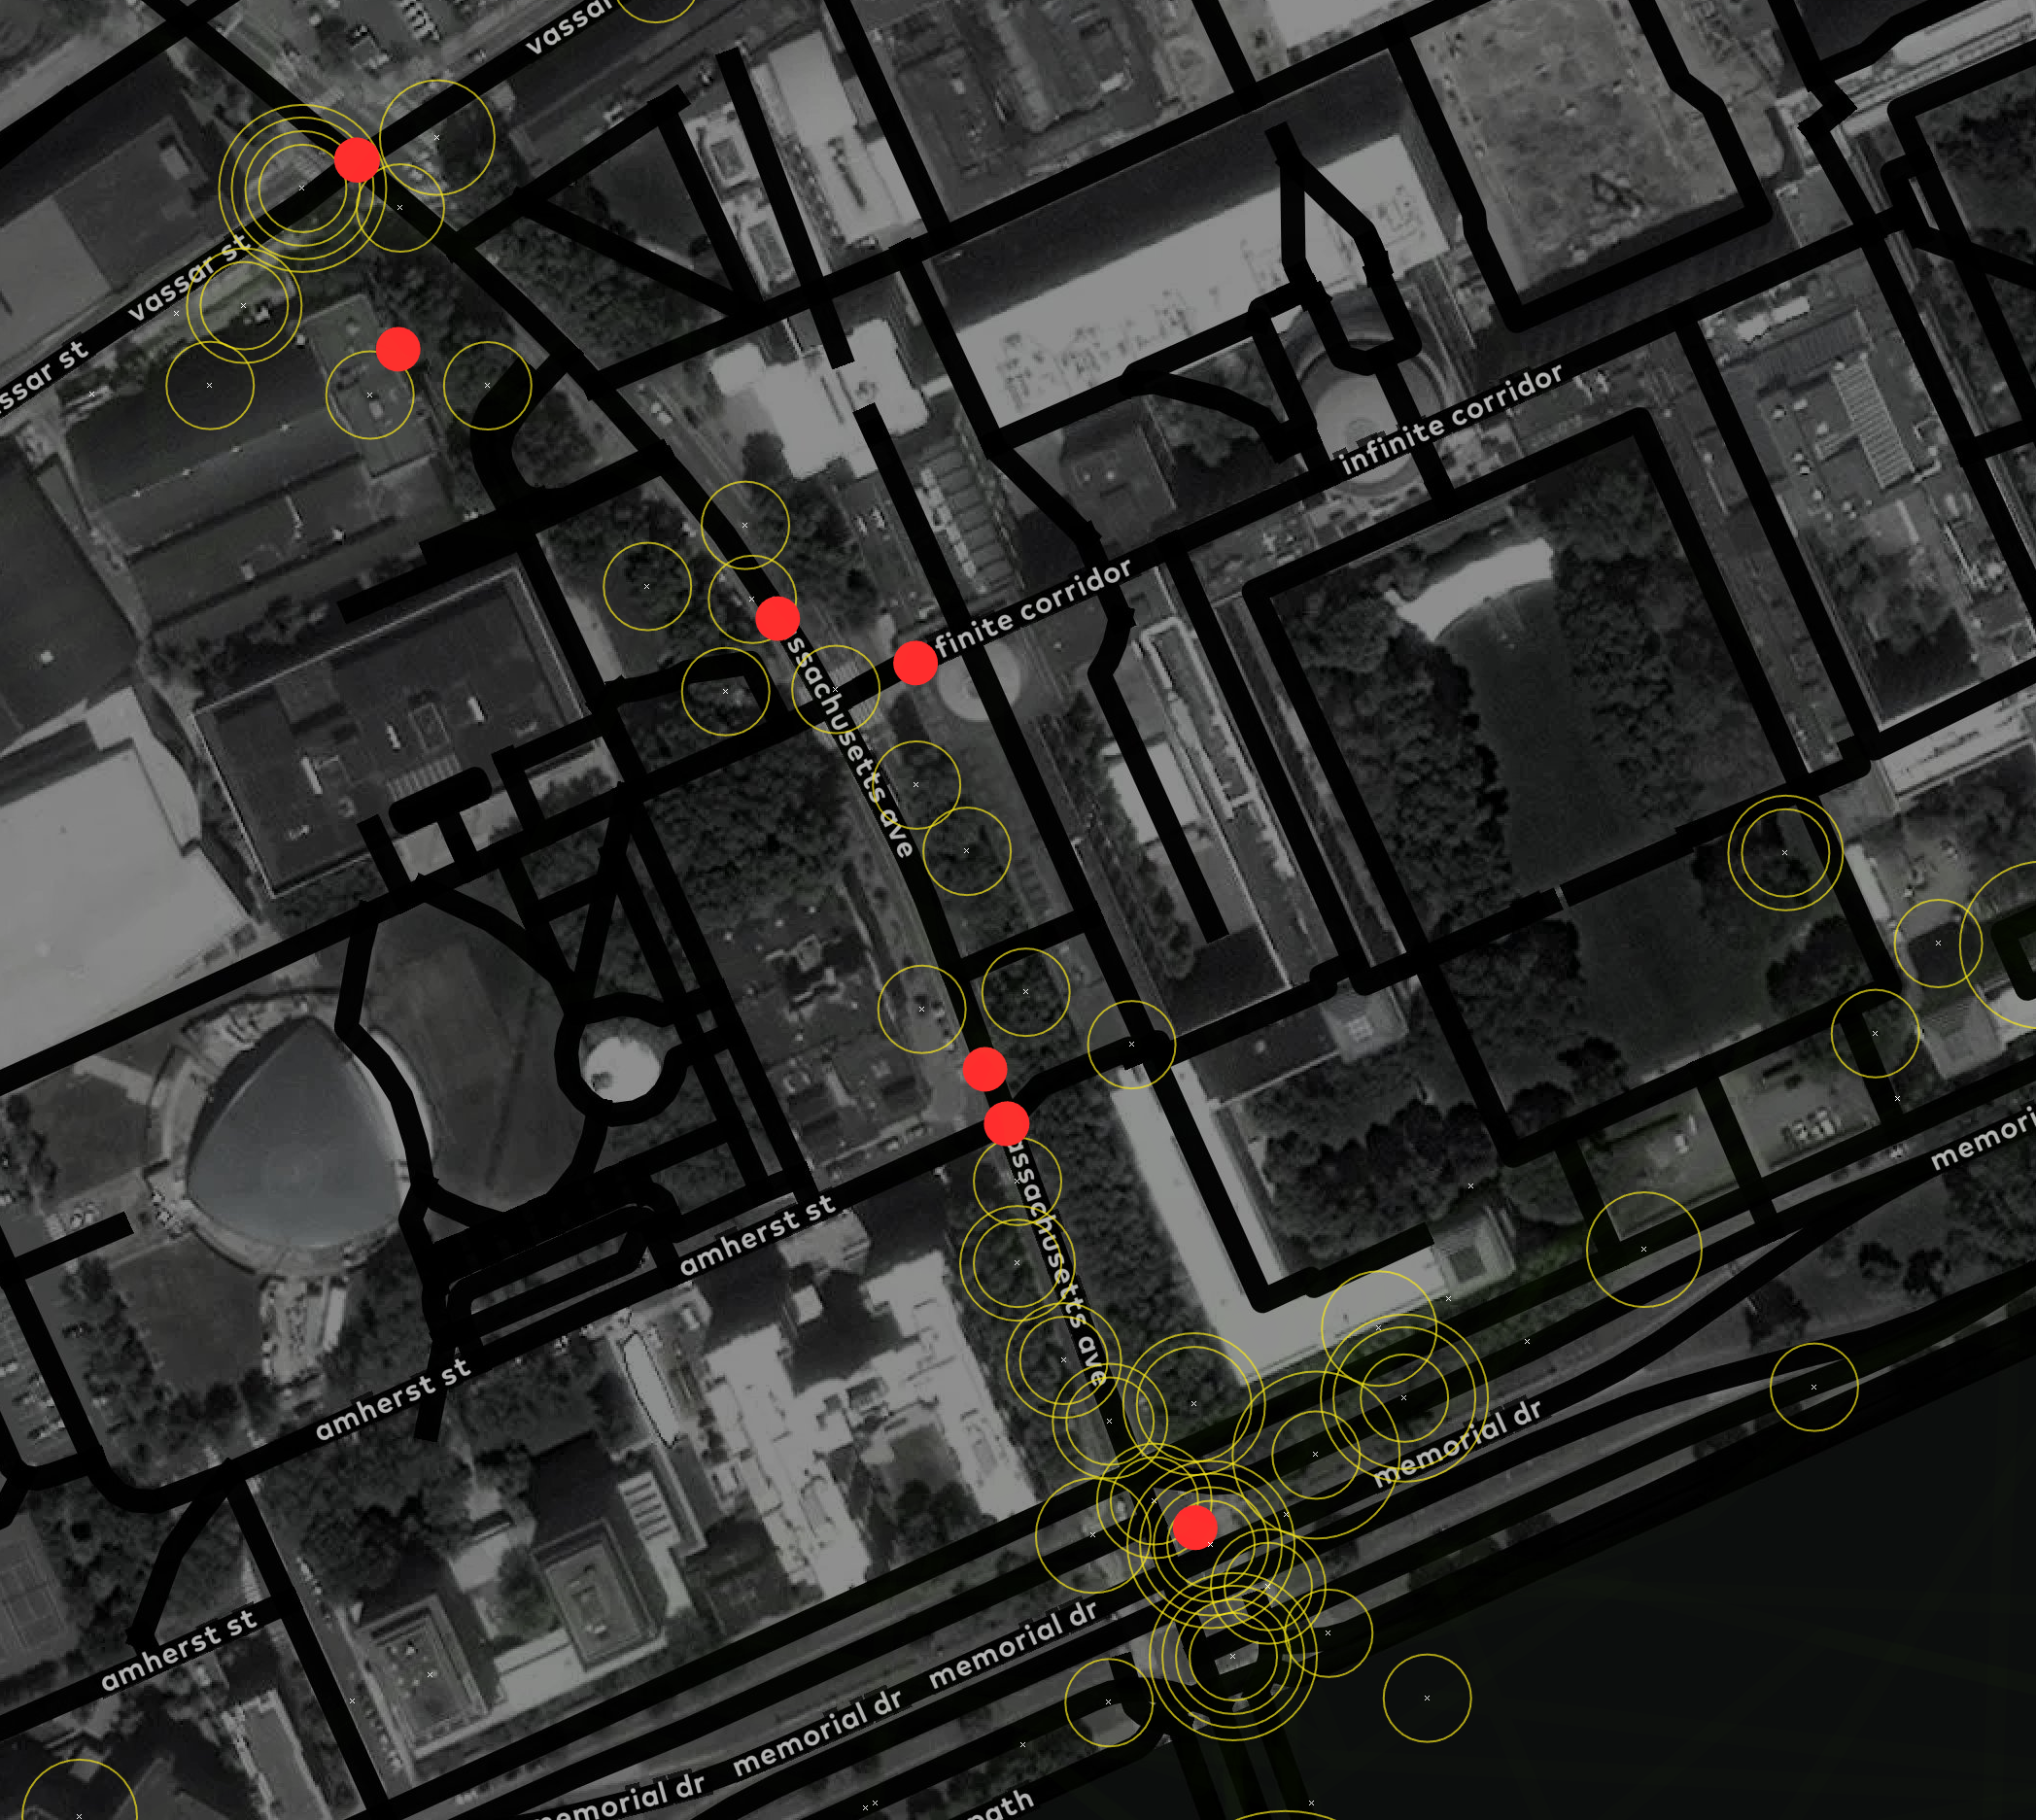
\includegraphics{appendix/B/fig/overlap_mass_avenue.png}               
  \caption[`bad' reports close to the entrance of MIT]{Withing the fixed route, this location tends to have the most pedestrians. The DING reports tend to concentrate at the entrance of the bridge, again having fast traffic passing close.}
  \label{fig:bad_mass}
\end{figure}

\begin{figure}[!htb]
  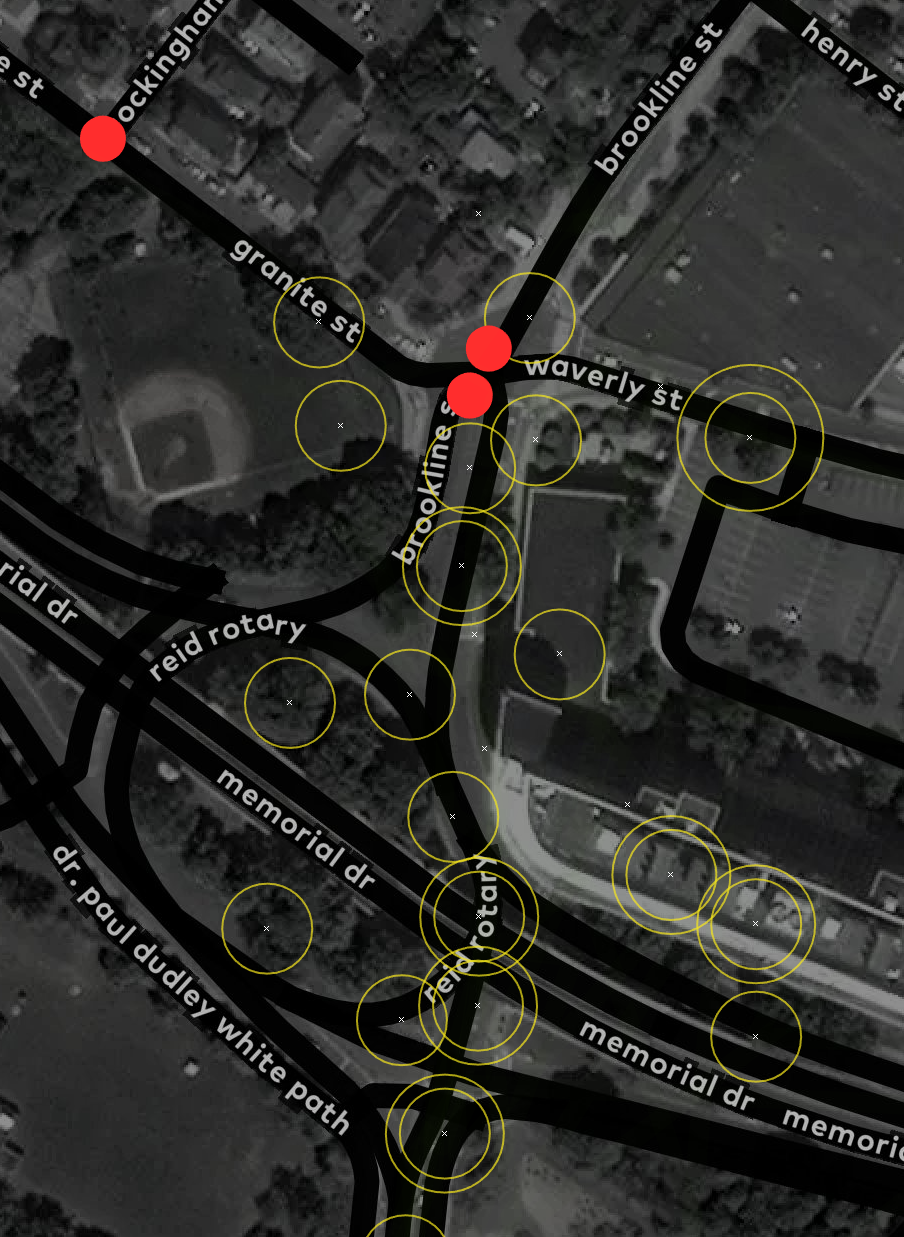
\includegraphics{appendix/B/fig/overlap_roundabout.png}               
  \caption[`bad' reports at the junction of BU bridge and memorial drive]{The end of BU bridge is a roundabout without street lights, totally dependant on eye contact. There is minimal road signs to indicate this is a shared lane with bikes and cars. This location was intended to be the most frightening location throughout the route, but turns out it was pleasant because the BU bridge car traffic shut down.}
  \label{fig:bad_roudabaout}
\end{figure}